\section{0514}\label{sec:0514}
\begin{questions}
    \question 输入是由数轴上的区间所组成的集合,这些区间由它们的两个端点表示。
    设计$O(n \log n)$算法识别所有包含在集合中其它某个区间的区间。
    这个问题与二维平面极大点问题有什么关系

    例如输入:$(1,3), (2,8), (4,6), (5,7), (7,9)$,则输出为$(4,6)$和$(5,7)$

    \begin{solution}


        \textsf{极大点的定义} \quad
        {
            \kaishu
            设$p_1=(x_1,y_1)$和$p_2=(x_2,y_2)$是平面上的两个点,
            如果$x_1 \le x_2$并且$y_1 \le y_2$,则称$p_2$支配$p_1$,记为$p_1 \prec p_2$。
            点集$S$中的点$p$为极大点,意味着在$S$中找不到一个点$q$,$q \ne p$并且$p \prec q$,
            即$p$不被$S$中其它点支配。
        }

        区间$(x_1, y_1)$包含区间$(x_2, y_2)$当且仅当\[
            x_1 \le x_2 \wedge y_1 \ge y_2
        \]

        将区间用平面上的点表示,所有的点都在直线$y=x$上方。

        \begin{figure}[H]
            \centering
            \begin{subfigure}[b]{0.45\textwidth}
                \centering
                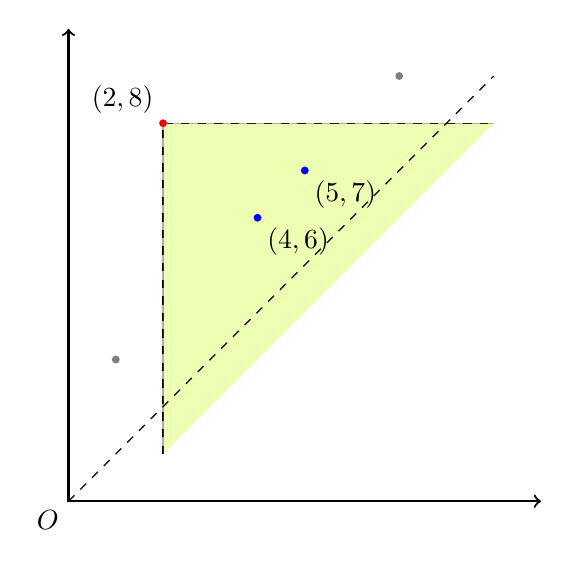
\begin{tikzpicture}[scale=0.6]
                    \coordinate (p1) at (1,3);
                    \coordinate (p2) at (2,8);
                    \coordinate (p3) at (4,6);
                    \coordinate (p4) at (5,7);
                    \coordinate (p5) at (7,9);

                    \draw[dashed] (2,1) -- (2,8) -- (9,8);
                    \draw[fill=lime, opacity=0.3] (2,1) -- (2,8) -- (9,8);

                    \filldraw [gray] (p1) circle (2pt);
                    \filldraw [red ] (p2) circle (2pt);
                    \filldraw [blue] (p3) circle (2pt);
                    \filldraw [blue] (p4) circle (2pt);
                    \filldraw [gray] (p5) circle (2pt);

                    \node [above left ] at (p2) {$(2,8)$};
                    \node [below right] at (p3) {$(4,6)$};
                    \node [below right] at (p4) {$(5,7)$};
                    \node [below left] at (0,0) {$O$};

                    \draw[thick, <->] (0,10) -- (0,0) -- (10,00);
                    \draw[dashed] (0,0) -- (9,9);
                \end{tikzpicture}
                \caption{$(x,y) \longmapsto (x,y)$}
            \end{subfigure}
            \begin{subfigure}[b]{0.45\textwidth}
                \centering
                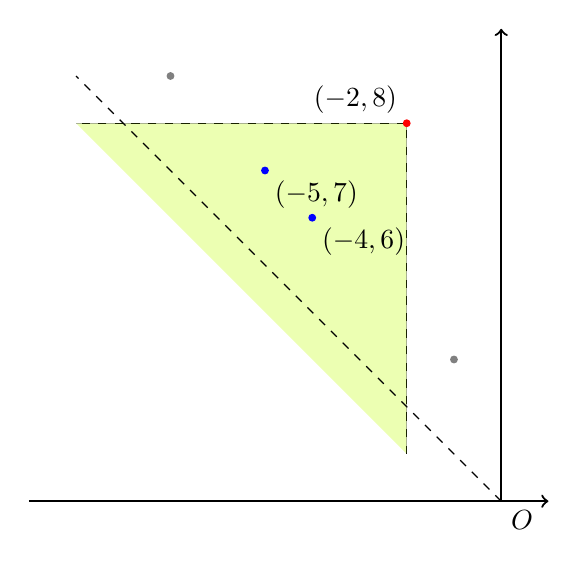
\begin{tikzpicture}[scale=0.6]
                    \coordinate (p1) at (-1,3);
                    \coordinate (p2) at (-2,8);
                    \coordinate (p3) at (-4,6);
                    \coordinate (p4) at (-5,7);
                    \coordinate (p5) at (-7,9);

                    \draw[dashed] (-2,1) -- (-2,8) -- (-9,8);
                    \draw[fill=lime, opacity=0.3] (-2,1) -- (-2,8) -- (-9,8);

                    \filldraw [gray] (p1) circle (2pt);
                    \filldraw [red ] (p2) circle (2pt);
                    \filldraw [blue] (p3) circle (2pt);
                    \filldraw [blue] (p4) circle (2pt);
                    \filldraw [gray] (p5) circle (2pt);

                    \node [above left ] at (p2) {$(-2,8)$};
                    \node [below right] at (p3) {$(-4,6)$};
                    \node [below right] at (p4) {$(-5,7)$};
                    \node [below right] at (0,0) {$O$};

                    \draw[thick, ->] (0,0) -- (0,10);
                    \draw[thick, ->] (-10,0) -- (1,0);
                    \draw[dashed] (0,0) -- (-9,9);
                \end{tikzpicture}
                \caption{$(x,y) \longmapsto (-x,y)$}
            \end{subfigure}
            \caption{将区间映射到二维平面上的点}
        \end{figure}

        为了与二维平面上极大点的定义相匹配,定义区间$(x,y)$映射到平面上的一点$(-x,y)$。
        则上述区间包含的等价条件相应地变为
        \[
            (x_2, y_2) \subseteq (x_1, y_1)
            \Longleftrightarrow -x_2 \le -x_1  \wedge y_2 \le y_1
            \Longleftrightarrow (-x_2, y_2) \prec (-x_1, y_1)
        \]

        所以该问题等价于在平面点集中,找出被其他任何一个点支配的所有点。
        即将区间集合映射到二维平面上的点集之后,找出二维平面中所有极大点的补集即可。

    \end{solution}

    \question  证明Graham算法是求凸包问题的一种最优算法

    \begin{solution}
        在$n$个点中选取$k$个点按一定顺序构成凸包,可能有$P(n, k)$种结果。
        由于$k$是未知的,所以共有\[
            \sum_{k = 3}^{n} P(n,k)
        \]种可能性。
        任取其中一种,选中正确的凸包的概率为\[
            p = \frac{1}{\sum_{k = 3}^{n} P(n,k)}
        \]
        其信息量为
        \begin{align*}
            I = & - \log p = \log \left( \sum_{k = 3}^{n} P(n,k) \right)
            = \log \left( \sum_{k = 3}^{n} \frac{n!}{(n-k)!} \right)
            =  \log \left( n! \sum_{k = 3}^{n} \frac{1}{(n-k)!} \right)          \\
            =   & \log n! + \log \left(\sum_{k = 3}^{n} \frac{1}{(n-k)!} \right)
            =  O(n \log n)
        \end{align*}

        一次比较操作能提供的信息量为$\log 2$,所以凸包问题的信息论下界为$O(n \log n)$。

        Graham算法的时间复杂度为$O(n\log n)$,与信息论下界同阶,是最优算法。

    \end{solution}

    \question 证明如果存在时间复杂度为$O(T(n))$的两个$n \times n$下三角矩阵的乘法,
    则存在时间复杂度为$O(T(n)+n^2)$的任意两个$n \times n$矩阵相乘的算法。

    \begin{solution}
        令$E$为$n$阶单位阵。设$A,B,C$均为$n$阶方阵,且$C = AB$。
        则矩阵\[
            Q = \begin{pmatrix}
                E & O & O & O \\
                B & E & O & O \\
                O & A & E & O \\
                O & O & B & E
            \end{pmatrix}
        \]是$4n$阶的下三角方阵。则有
        \[
            Q^2 = \begin{pmatrix}
                E  & O  & O  & O \\
                2B & E  & O  & O \\
                AB & 2A & E  & O \\
                O  & BA & 2B & E
            \end{pmatrix}
        \]

        构造矩阵$Q$需要时间$(4n)^2$,作矩阵乘法需要时间$T(4n)$,取出$AB$的值需要时间$n^2$。

        因此该算法的时间复杂度为$O(T(4n) + 17n^2)$。
        在假设$T(cn) = T(n)$的条件下,该复杂度即为$O(T(n)+n^2)$。
    \end{solution}

    \question  如果在序列$x_1,x_2, \dots ,x_n$中,存在某个$i$使$x_i$是序列中的最小者,
    且序列\[ x_i,x_{i+1}, \dots ,x_n,x_1,\dots, x_{i-1} \]是递增的,
    则称序列$x_1,x_2, \dots ,x_n$是循环序列。
    设计算法找出循环序列中最小元素的位置。
    为简单起见,假设该位置是唯一的。
    证明你的算法是最优的。

    \begin{solution}
        遍历整个序列以寻找最小值的时间复杂度为$O(n)$。

        在$n$个数组中随机选取一个数,该数是序列中最小的值的概率为$p = 1 / n$,信息量为$\log n$。
        下面给出一种时间复杂度为$O(\log n)$的算法,该算法的时间复杂度达到了问题的信息论下界,是一个最优算法。

        若序列$\left\{x_i\right\}$是递增的,则$\forall i,j : i < j \rightarrow x_i < x_j$。
        所以,若$\exists i < j : x_i > x_j $,则该序列是非增的;
        又因为该序列是循环递增的,所以序列的极值点一定在$i,j$之间。

        \textbf{伪代码见算法\ref{alg:0514:4}}

        该算法类似于二分查找,每次搜索范围减半直到找到最小值,其时间复杂度为$O(\log n)$。

    \end{solution}

    \begin{algorithm}[!ht]
        \caption{循环递增序列的极值点}\label{alg:0514:4}
        \begin{algorithmic}[1]
            \Require {序列$x[1 \dots n]$}
            \Ensure {$\mathrm{argmin}_i x_i$}
            \State $left \gets 1, right \gets n$
            \If { $x[left] < x[right]$ }    \Comment{序列是有序的}
            \State \Return $left$
            \Else
            \Repeat
            \State $mid \gets \frac{left + right}{2}$
            \If { $x[mid] < x[right]$ }     \Comment{$(mid, right)$是有序的}
            \State $right \gets mid$
            \Else                           \Comment{$(left, mid)$是有序的}
            \State $left \gets mid$
            \EndIf
            \Until{$right - left \le 1$}
            \State \Return $right$
            \EndIf
        \end{algorithmic}
    \end{algorithm}

\end{questions}
